\section{Results}

\subsection{General Scaling laws}

To identify promising models for prompt tuning, we first benchmarked
different model families on a 20,000-sample training set from
MultiNERD. Results are shown in Table~\ref{tab:multinerd}. For all
models, fine-tuning and prompt tuning substantially outperformed the
few-shot baseline. For most model families, the two approaches
achieved comparable performance. Differences between random and
informed prompt initialisation were small.

\begin{table}[ht]
  \centering
  \footnotesize
  \setlength{\tabcolsep}{4pt}
  \renewcommand{\arraystretch}{0.9}
  \caption{
    MultiNERD test Macro-F1 (\%), trainable parameters, and virtual
    prompt length after three epochs on 20,000 English sentences. FT
    = fine-tuning; PT = prompt tuning (pre. = system-prompt
    initialisation, rand. = random initialisation); FS/head =
    five-shot prompting for decoders or an encoder classification
    head. %Bold indicates the highest F1 in each column.
  }
  \label{tab:multinerd}
  \begin{tabular}{lrrrrrrrr}
    \toprule
    Model     & Instructable & Params & PT params & FT          & PT (pre.)   & PT (rand.)  & FS/head & Prompt tokens \\
    \midrule
    mmBERT    & No           & 307M   & 23K       & \textbf{91} & 88          & 73          & 14      & 15 \\
    Gemma 3   & Yes          & 4.3B   & 145K      & \textbf{86} & 73          & 74          & 43      & 57 \\
    Llama 3.1 & Yes          & 8B     & 237K      & 81          & \textbf{88} & 79          & 52      & 58 \\
    Qwen 3.5  & Yes          & 9B     & 241K      & \textbf{84} & 83          & \textbf{84} & 64      & 59 \\
    \bottomrule
  \end{tabular}
\end{table}

Figure~\ref{fig:multinerd-scaling} shows how performance changes with
the number of available training samples. F1 score generally improves
with increasing training-set size. Prompt tuning tends to perform
better with limited training data, whereas fine-tuning can surpass it
as the dataset grows. Across all models, 1,000 training examples were
sufficient to reach near-optimal performance, with only modest
improvements thereafter.

\begin{figure}[ht]
  \centering
  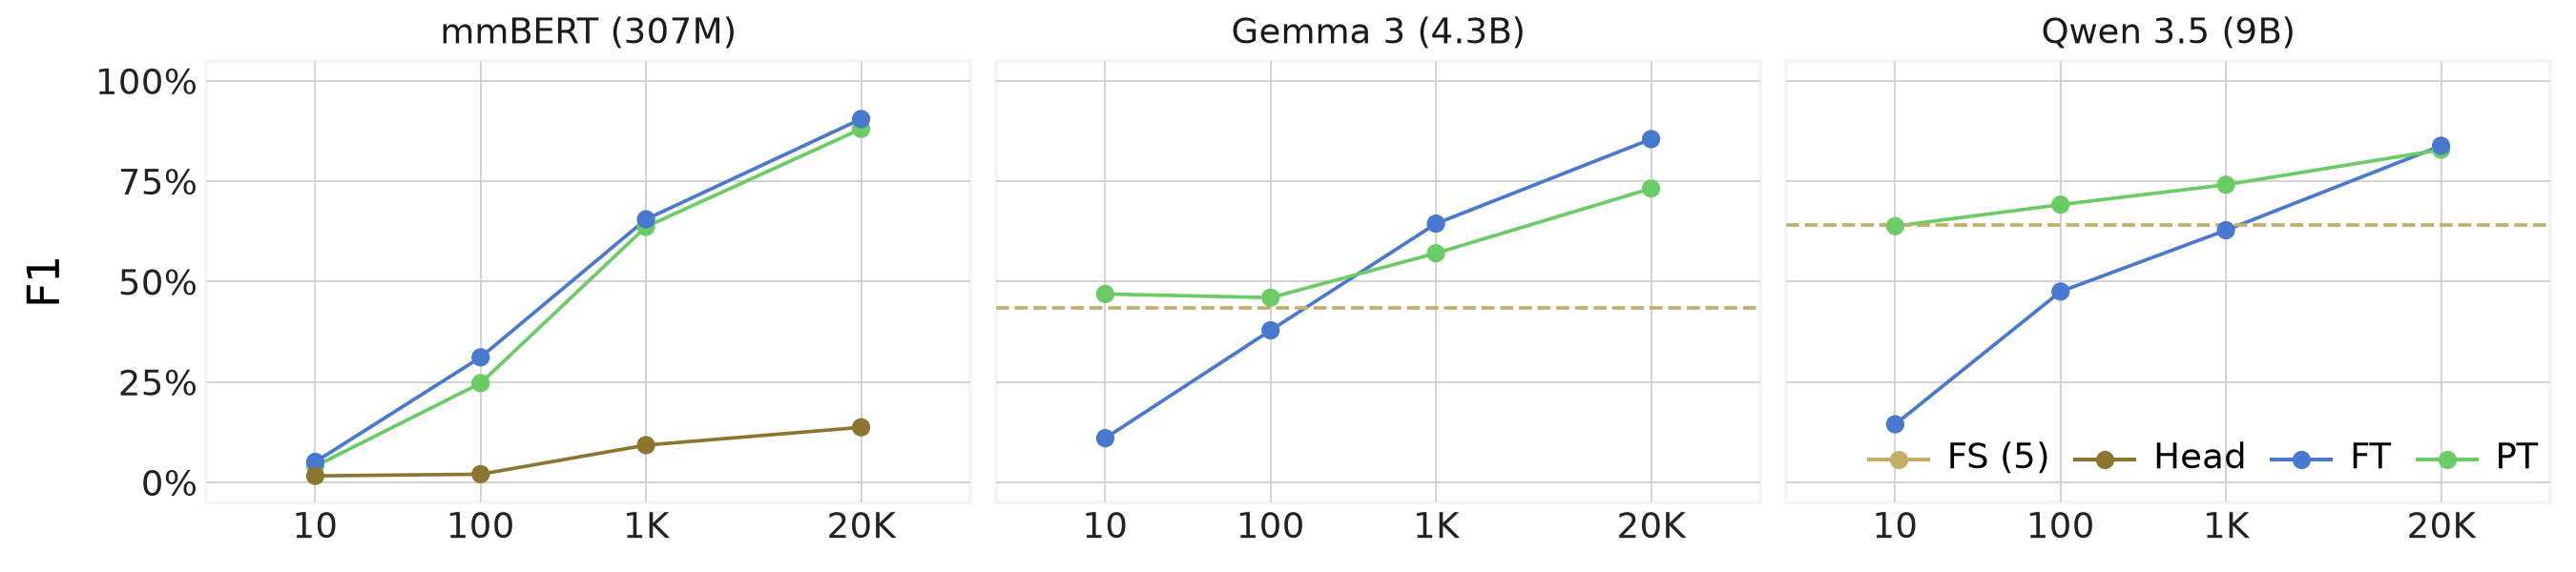
\includegraphics[width=\textwidth]{fig/multinerd-data-scaling.png}
  \caption{
    MultiNERD test Macro-F1 (\%) by number of labelled training
    sentences. FT = fine-tuning; PT = prompt tuning; Head = encoder
    classification head and FS (5) = five-shot prompting as baselines.
  }
  \label{fig:multinerd-scaling}
\end{figure}

\subsection{Performance on Drug Discontinuation Data}

Figure~\ref{fig:eh30-scaling} shows how performance changes with the
number of annotated phrases. Prompt tuning did not outperform the
baseline for mmBERT, possibly due to limited capacity for instruction
following in the Estonian medical domain. In contrast, it clearly
outperformed fine-tuning for the other two models. Occasional drops
in performance likely reflect statistical instability, as the smaller
training sets provide insufficient data to offset the effects of
unrepresentative samples.

\begin{figure}[ht]
  \centering
  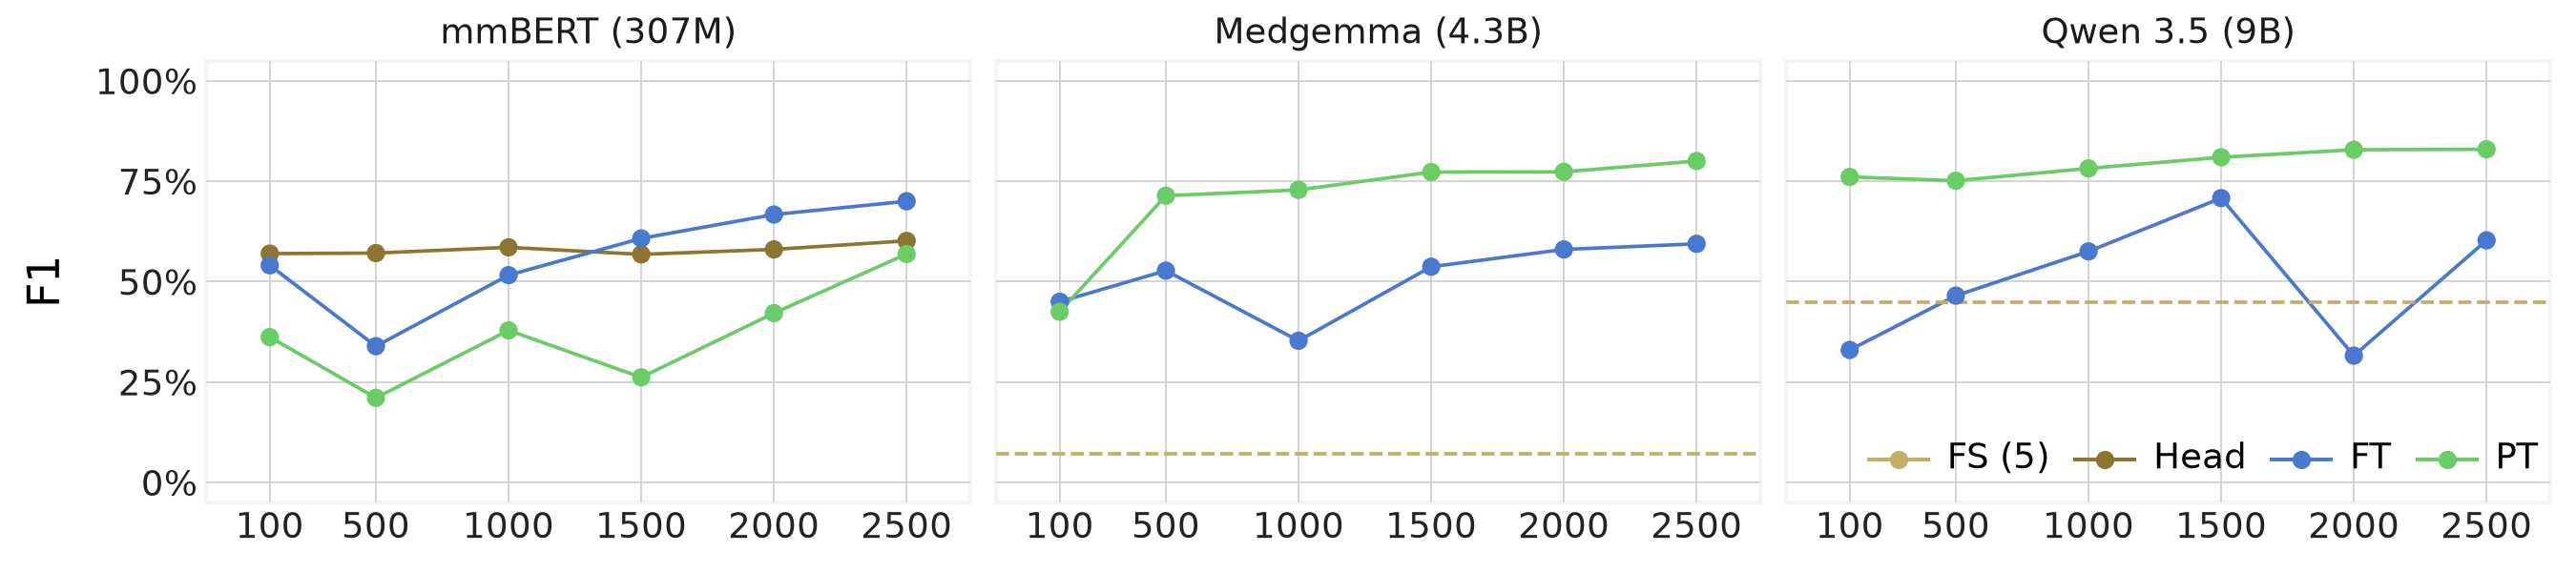
\includegraphics[width=\textwidth]{fig/eh30-data-scaling.png}
  \caption{
    Estonian medication-discontinuation test F1 (\%) by training-set
    size, measured as the number of labelled anamnesis notes and
    evaluated on a fixed test split. FT = fine-tuning; PT = prompt
    tuning; Head = encoder classification head; FS (5) = five-shot
    prompting, shown as a fixed decoder baseline.
  }
  \label{fig:eh30-scaling}
\end{figure}
